\section{System's Perspective} 

\subsection{MiniTwit Application}
%Should contain a description and illustration of the design and architecture of our ITU-MiniTwit system.

%- What is our overarching architecture?
%- Have we made any design choices?
%- How is this best illustrated? Diagram?

%terraform og hvordan det bør sættes op?

We chose to rewrite the MiniTwit application to C\#, which has a nice web framework, Blazor WebAssembly, that allows us to write all our code using the same language. Blazor additionally runs as a single-page application which is faster at loading, partly because data can be fetched in the background and because full-page reloads are rare. One downside of WebAssembly is the long initial load of the application, which hopefully can be reduced or removed with future versions of .NET.
Our application depends on a few NuGet packages to communicate with the rest of the system.

\begin{center}
\begin{tabular}{|c|p{0.6\linewidth}|}
    \hline
    Identity Server & An easy and secure way of managing users. \\
    \hline
    Prometheus-net & Sets up the /metrics endpoints for Prometheus. \\
    \hline
    Serilog.Sinks.ElasticSearch & Gives Serilog a log sink for ElasticSearch, letting it send logs directly to ElasticSearch \\
    \hline
    EF Core & O/RM for communicating with the database\\
    \hline
\end{tabular}
\end{center}

\noindent We aimed for our system to have a simple and maintainable architecture, by utilizing as few different tools as possible and by using software architectural patterns. The patterns we chose to strive for have been Clean Architecture, Repository Pattern, and Client-Server. We use several other patterns too, but we don't consider them something we strive for, as they are simply a byproduct of the tools and framework we use. 

\begin{wrapfigure}{r}{0.4\textwidth}
    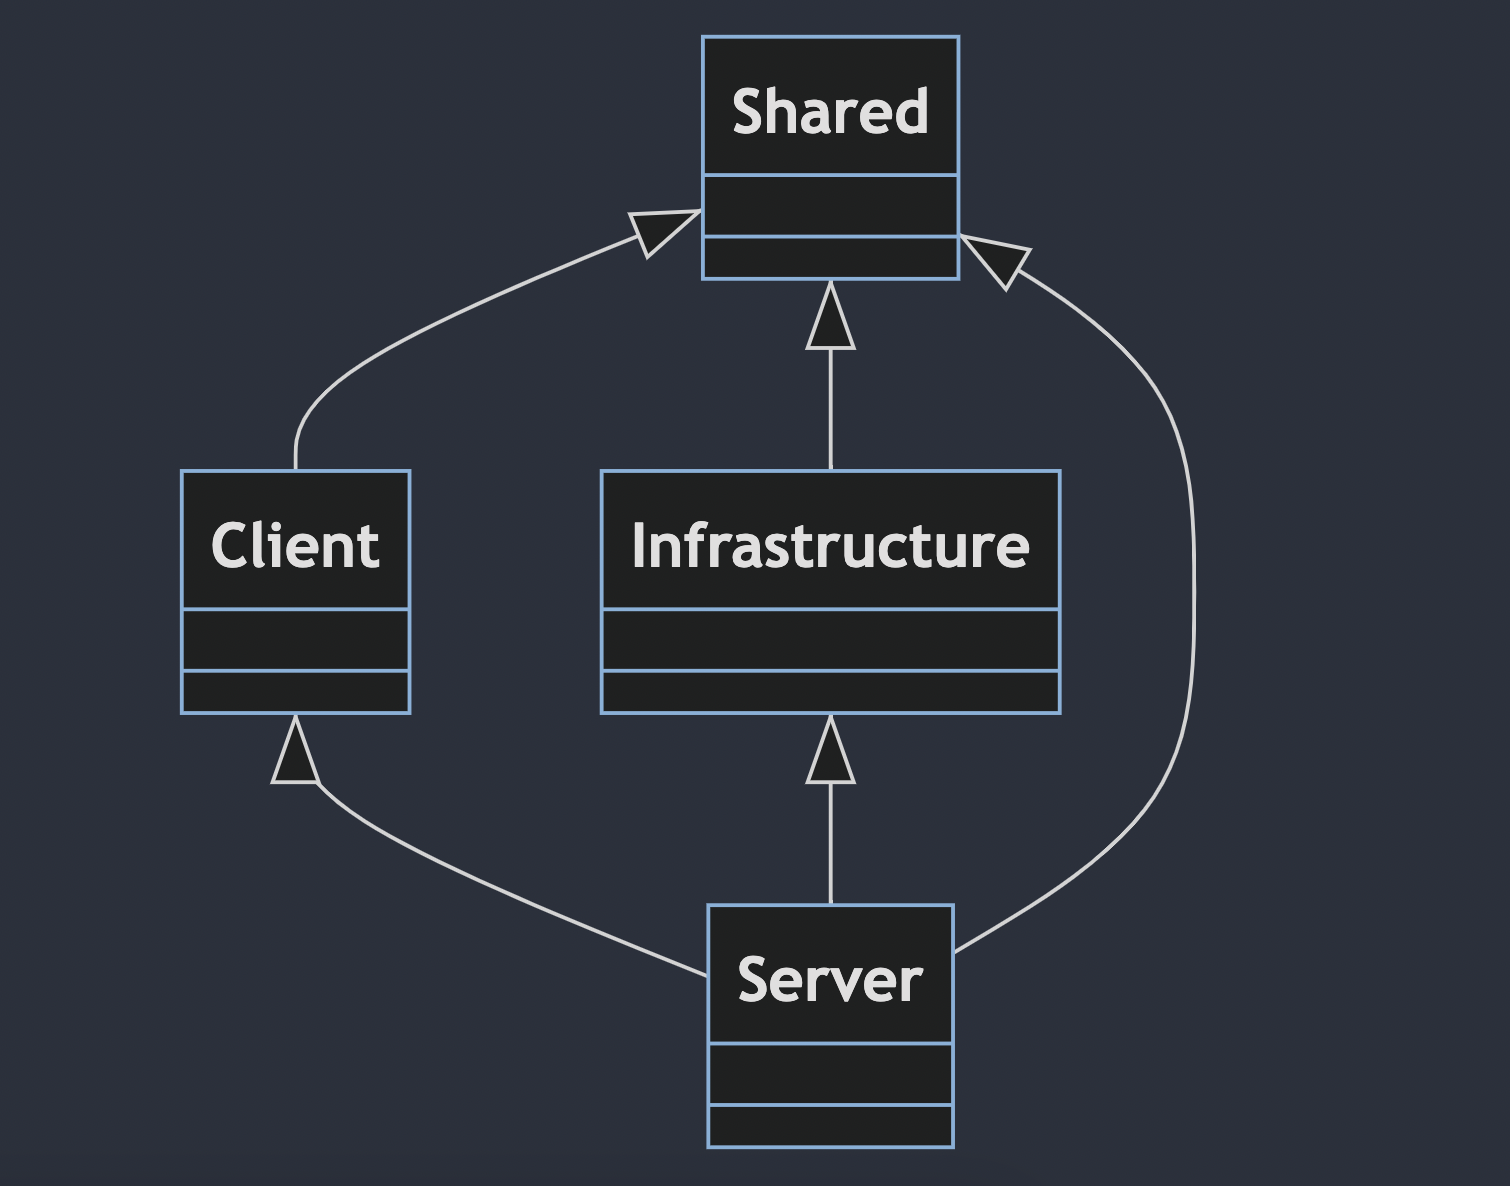
\includegraphics[width=0.9\linewidth]{Images/onionStructure.png} 
    \caption{Project Architecture}
    \label{fig:projectDependencyGraph}
\end{wrapfigure}

\texttt{Clean architecture} gives us separation of concern and greater modularity. We achieve this by having our code split into 4 C\# projects. One project, \texttt{Shared}, is for our data transfer objects (\texttt{DTO's}) and repository interfaces, so we will be able to mock our repositories without a dependency on them. A second project, \texttt{Infrastructure}, is for the repositories, database context, and models for the database schema, where the repositories depend on the \texttt{Shared} project. The third project, \texttt{Client}, contains the \texttt{Blazor} files, responsible for the presentation layer and user interface. Finally, the fourth project, \texttt{Server}, is the actual server that contains the API controllers, serves the frontend, and the application configuration. The controllers have a dependency on \texttt{Infrastructure} and \texttt{Shared}, as the controllers need the repositories and the DTO's. For the \texttt{Server} to serve the frontend it has a dependency on the \texttt{Client}. Thus none of our projects are mutually dependent and the core is the \texttt{Shared} project, from where it aggravates outward to a layer containing the \texttt{Infrastructure} and \texttt{Client}. Lastly a layer with the \texttt{Server} as the part that other systems can interact with.

We use a \texttt{Repository pattern} to add abstraction around our communication with the database. Even though we use EF core which some would say is enough abstraction, then repositories allow us to make a switch over to use something like \texttt{Dapper} instead of \texttt{EF Core}.

\subsubsection{API request route}
The route of data in our application starts with the user. When a user sends a request to the server, then it needs to pass through a few places before coming back to the user. Below is a sequence diagram illustrating the journey of an arbitrary request along its designated 'route'.

\vspace{3pt}
\begin{figure}[H]
    \centering
    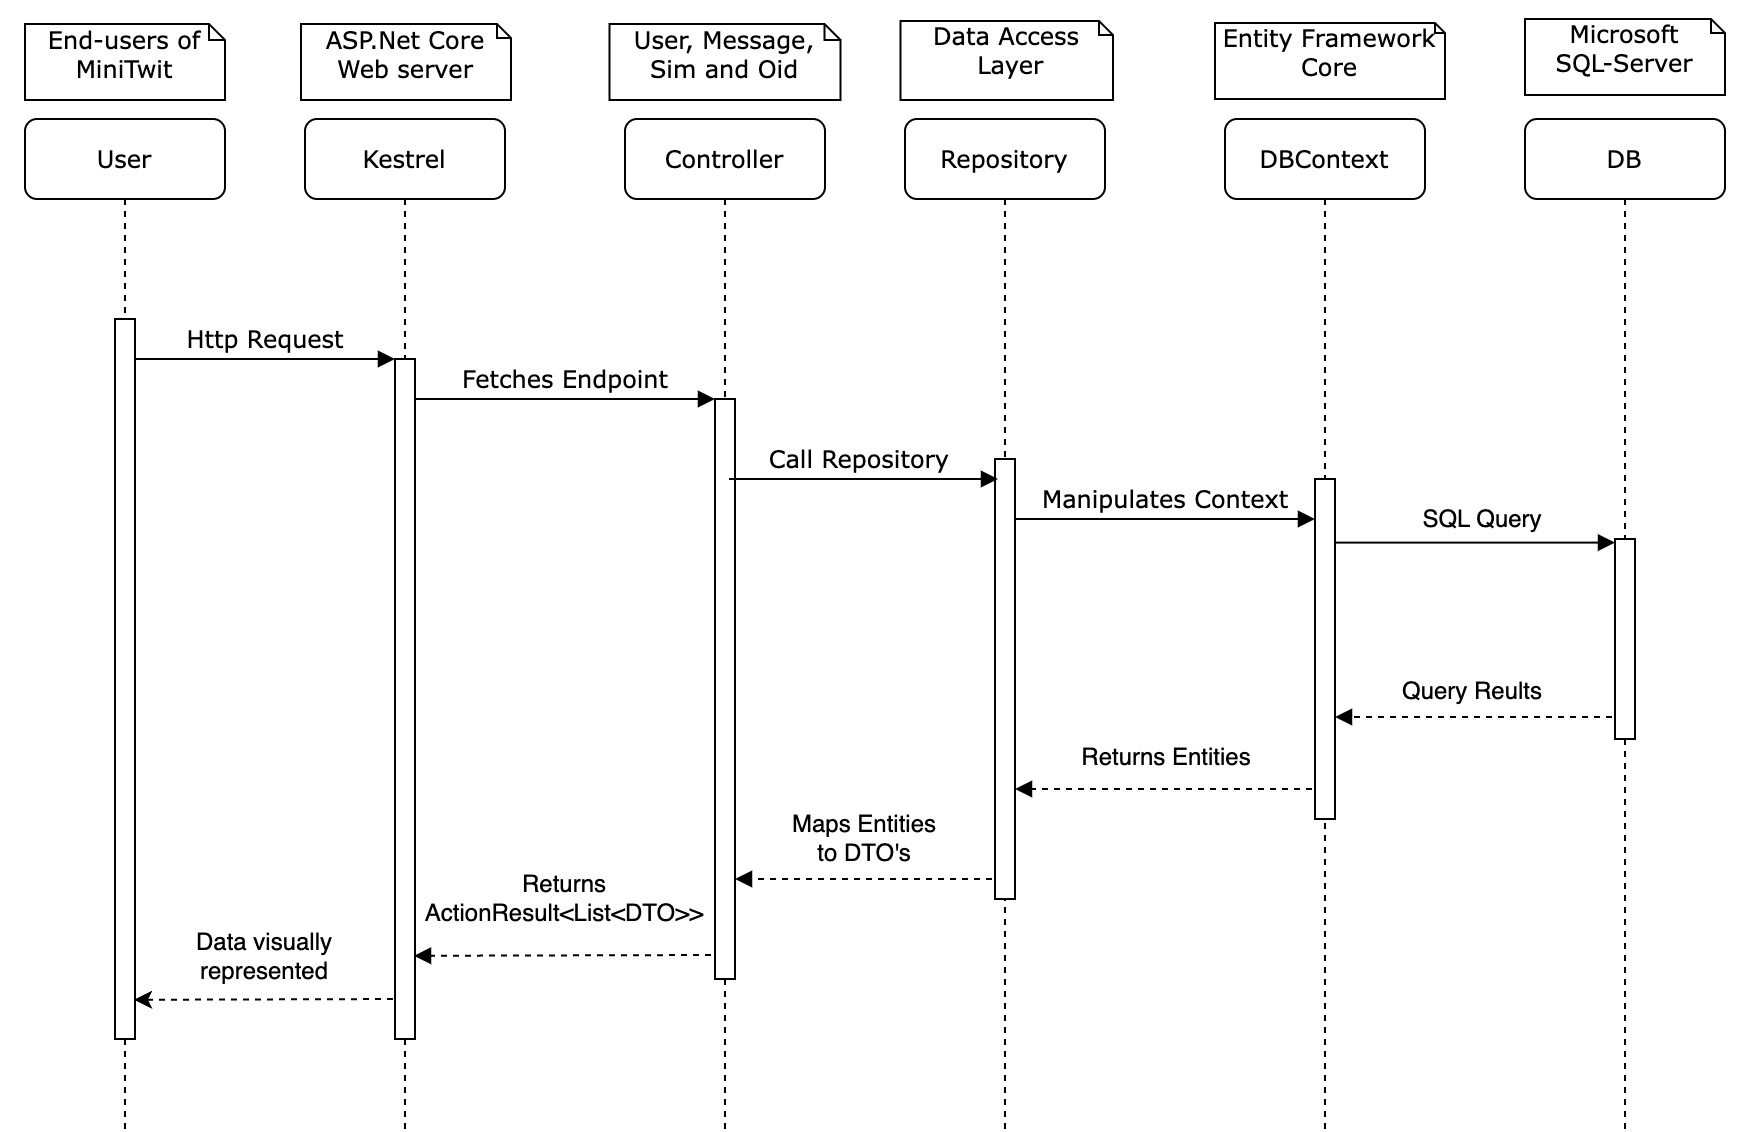
\includegraphics[width=0.65\linewidth]{Report/Images/SequenceDevOps.jpg} 
    \caption{Data journey}
    \label{fig:API_Sequence}
\end{figure}
\vspace{3pt}

The route starts with the user sending a request to the server. On the server, Kestrel, the web server, receives the request and sends it to the controller method that matches the endpoint the request targeted. The controller then uses one of the repositories, that asks EF Core to format a query and send it to the database. When the database returns data then it aggravates up the ladder again and back to the user.

\subsubsection{Database}
\noindent For the server to communicate with the database we chose to use the popular open-source O/RM Entity Framework Core, also known as EF Core. EF Core makes it possible to define the database schemas and maintain the database state. Additionally, it removes the type barriers between code and database while making it possible to query the database without writing SQL, which blocks SQL injection.

\subsubsection{Dependencies}
%explain the NuGet and pagage dependencies
At a low level of abstraction, our application has specific dependencies such as libraries and packages. These dependencies are internally within our program and are imported and installed using dotnet as NuGet packages. A visual representation of package dependencies for our application can be seen in figure \ref{fig:packageDependencyGraph}. 

\begin{figure}[H]
    \centering
    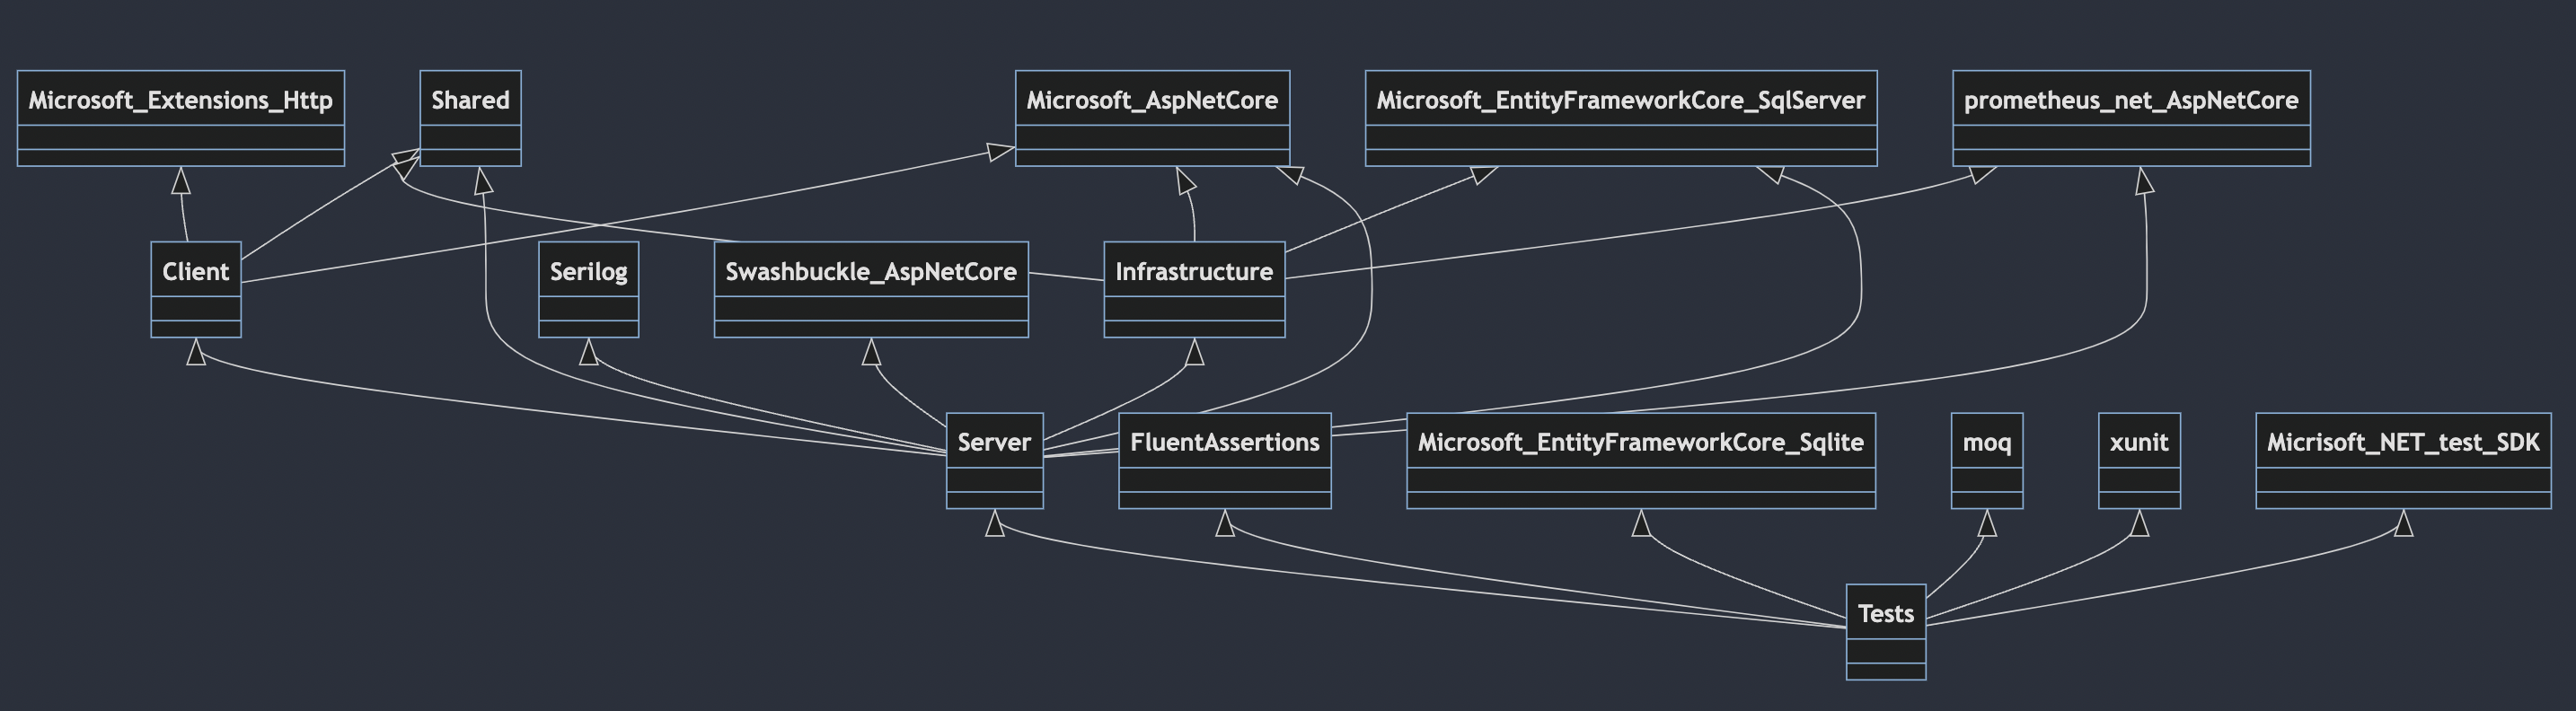
\includegraphics[width = \textwidth]{Images/dependencies2.png}
    \caption{Package dependency graph for C\# application}
    \label{fig:packageDependencyGraph}
    \centering
\end{figure}

\subsection{Tools \& Expanded System Architecture}

This section briefly describes the different tools the system utilizes, and for what purpose. Most are talked about in further detail in the Proces' Perspective section. Figure  \ref{fig:infrastructureDependencyGrapg} shows an overview of the infrastructure and dependencies of the system and its tools. 

\begin{figure}[H]
    \centering
    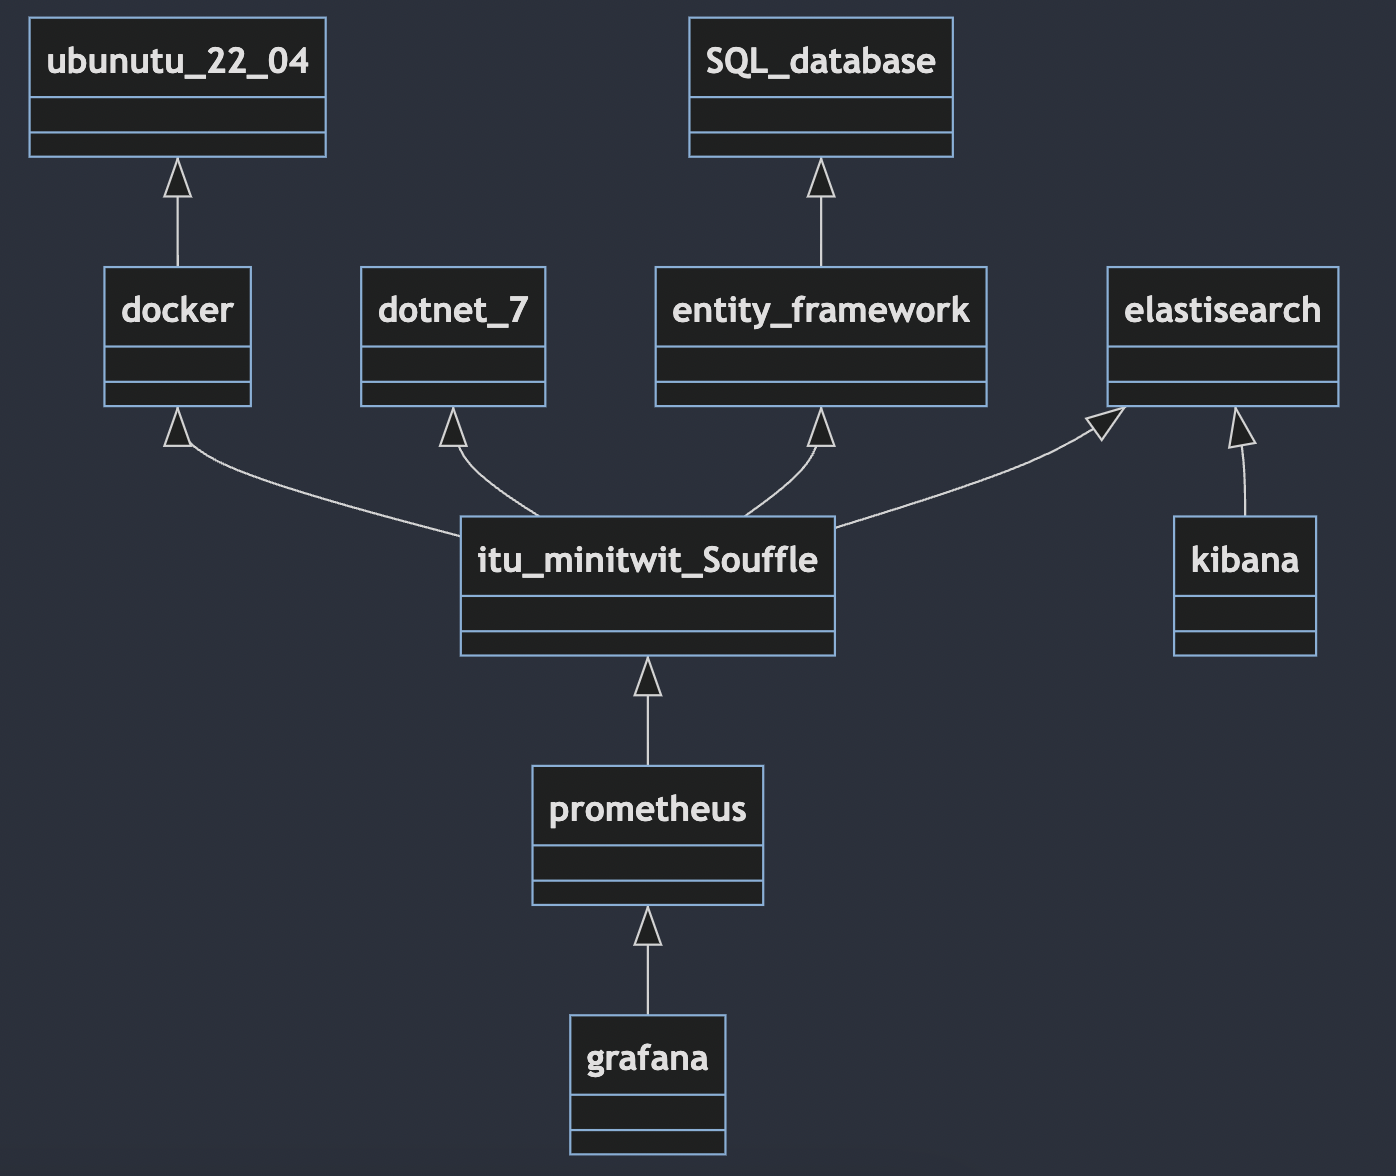
\includegraphics[width = 0.6\textwidth]{Images/application_dependencies.png}
    \caption{Infrastructure dependency graph}
    \label{fig:infrastructureDependencyGrapg}
    \centering
\end{figure}


\subsubsection{.NET 7}
This is the platform our project is built on. We chose this runtime since it is the one we are most familiar with and it contains a lot of libraries that suits our needs. 

\subsubsection{Docker \& Ubuntu 22.04}
Docker is responsible for building, shipping, and running our application through containers. It makes it possible to have complete control of the environment in which programs must run (we use Ubuntu 22.04), which simplifies compatibility. Docker Swarm also enables scaling of the system within virtual machines.

\subsubsection{Digital Ocean}
As recommended, Digital Ocean is our chosen provider of cloud infrastructure. It is user-friendly and makes controlling our domain name simple by allowing it to be routed through Digital Oceans NS records. However, as providers go, it is expensive. We had a limited amount of free credits, but we were restricted in the number of virtual machines we could afford. Our system has 2 droplets; one for our server, and one for all our tools. We would have preferred to separate our tools on individual droplets, potentially managed as a swarm for easy balancing, but it was not possible on our budget. 

\subsubsection{GitHub Actions}
GitHub Actions allows us to integrate our workflows, and apply our tools to our branches before merging them together, ensuring a certain level of quality control. E.g. by integrating testing as a prerequisite before merging code changes.

\subsubsection{Prometheus \& Grafana}
Prometheus is responsible for monitoring our system by periodically querying its specified metric endpoints for data. This data is then accessed by Grafana, which is the platform responsible for visualizing it on its dashboards. See \ref{Monitoring} for more detailed information.

\subsubsection{Superlinter \& Snyk}
Lint Code Base (SuperLinter) is a static analysis tool we use to identify and reduce possible code smells, such as duplicated code segments and long methods since these smells may affect the maintainability and readability of the code. The SuperLinter was chosen for its versatility, as it includes pre-configured linters for multiple languages and allows easy customization to align with our project's specific requirements.

Snyk is another static analysis tool we use due to its ability to identify and address security vulnerabilities. It scans open-source libraries and dependencies, ensuring our code is as robust and secure as possible.

\subsubsection{ElasticSearch \& Kibana}
ElasticSearch is a search and analytics engine that enables accurate, and near real-time searching of data, allowing rapid data retrieval and analysis, which makes it perfect for reading aggregated system logs. Though it is scalable and distributable, we only run one instance of it, even though it means we lose the redundancy. Kibana on the other hand is a data visualization and exploration tool that allows for the creation of dashboards to analyze and present data. 

Together these tools store, search, analyze, and visualize log data in our MiniTwit system. See \ref{Logging} for more details.

\subsection{Reflection of System State}

DevOps is a crammed course. It has not been possible to implement everything. These are the tools the current system does not have, either because it was skipped, down-prioritized, or seemingly incompatible with our setup.  

\subsubsection{Terraform}
This was never set up. We had a hard time understanding how the system should be set up and what parts of our infrastructure it should manage. Our rough understanding is that it could have made it easy to switch cloud providers and scale the number of machines the system should be distributed on. 

\subsubsection{NGINX in the Swarm}
We have made a script that allows us to pass in a few addresses of VM's, and then have our Server deployed with an NGINX load balancer in front. We have had some issues with loading times when going through the load balancer to the servers though.  

\subsubsection{Sonarqube \& Code Climate}
We never set up SonarQube and CodeClimate in our project due to time limitations. Theoretically, these static analysis tools would detect bugs, vulnerabilities, and code smells in order to improve code quality. Since we already implemented the Superlinter and Snyk we decided to down-prioritize these tools.

\subsection{License}
%Describe briefly, if the license that we have chosen for our project is actually compatible with the licenses of all our direct dependencies. 

We chose the GNU General Public License v.3.0 (GPL-3.0). As it is more restrictive in future third-party usage than the MIT license, while remaining compatible with our tools, and promoting collaboration with the development community.

\begin{itemize}
    \item Docker, Snyk, Grafana and Prometheus is distributed under the Apache License 2.0, which is compatible with GPL-3.0.
    \item Kibana and ElasticSearch are licensed under the Elastic License, which has some limitations that we are in accordance with.
    \item .NET and Superlinter is under the MIT License, which is compatible with GPL-3.0.
    \item NGINX is available under the NGINX Open Source License, which is compatible with GPL-3.0.
    \item Ubuntu is itself released under GPL.
    \item Identity Server has an open and free license while we don't sell our software or our services.
    \item Terraform is under the MPL 2.0 license, which is compatible as long as we do not distribute their source code.
\end{itemize}
